\documentclass[a4paper,12pt]{report}
\usepackage[utf8]{inputenc}
\usepackage{amsmath}
\usepackage{amssymb}
\usepackage{amssymb}
\usepackage{graphicx}
\usepackage{hyperref}
\usepackage{caption}
\usepackage{geometry}
\usepackage{lmodern}
\usepackage{tikz}
\usepackage{tabularx}
\usepackage{hyperref}
\usepackage{mathtools}
% \usepackage{colorlinks=true,linkcolor=blue}
% Définition des marges
\geometry{left=1.5cm, right=2cm, top=1.5cm, bottom=1.5cm}

\newtheorem{theorem}{Theorem}
\newtheorem{definition}{Definition}
\newtheorem{example}{Example}
\newtheorem{remark}{Remark}
\newtheorem{corollary}{Corollary}
\newtheorem{lemma}{Lemma}
\newtheorem{proposition}{Proposition}
\newtheorem{proof}{Proof}

%%%%%%%%%%%%%%%%%%%%%%%%%%%%%%%%%%%%%%%%%%%%%%%%%%%%%%
\begin{document}

% \hspace{-1cm}{\includegraphics[scale=0.3]{Image/logo_ufr_mathinfo.png}} \hfill
% \raisebox{1.2cm}{\begin{minipage}[t]{0.3\textwidth}
%   {\includegraphics[scale=0.45]{Image/udsTransparent.png}} % Remplacez par le chemin de votre autre image
  
%   {\includegraphics[scale=0.45]{Image/Inria-logo.png}}
% \end{minipage}}



\begin{center}
  \raisebox{-1cm}{ % Ajustez la valeur pour déplacer le minipage verticalement
          \begin{minipage}[c]{10cm}
              \centering \bf
              \bf\Large Computational Mechanics and Poromechanics for Induced Seismicity and Control\\
              % UFR of Mathematiques and Informatique\\
              % Departement of Mathematique 
          \end{minipage}
      } 
\end{center}

\vglue5mm
% \centering\vglue3cm\sl
\vspace{1cm}
% \centering
\begin{center}
  \underline{\bf\Large Doctoral Candidate Challenge – ERC INJECT Project} \\
  % \underline{\bf\Large Innovation Modeling (CSMMaster’s in Scientific Computing andI)}
\end{center}
\vglue1mm
\vspace{0cm}
\begin{center}
\vskip1mm
\setlength{\fboxsep}{18pt} % Ajustez l'espace entre le contenu et le bord de la boîte
\setlength{\fboxrule}{2pt} % Ajustez l'épaisseur du bord de la boîte

\fbox{
            \begin{minipage}{\textwidth}
                \centering
                \textbf{\Large COUPLED THERMO–HYDRAULIC ANALYSIS OF A 2-D GEOTHERMAL RESERVOIR}
            \end{minipage}
        }
\end{center}
\vglue5mm
\vskip5mm
\vspace{0.2cm}
\vfill
\begin{minipage}[t]{10cm}
\hspace{0.7cm}{\underline{\bf  Presented by:}\\[3mm]} \bf
CHAHID RAHOUTI\\
\end{minipage}
\hfill
\begin{minipage}[t]{5cm}
\underline{\bf Supervised by:}\\[4mm]\bf
\hfill Dr.L0ANNIS   \\ STEFANOU
\end{minipage}
\vfill
\vfill
% \centering
\begin{center}
  \today
\end{center}

%%%%%%%%%%%%%%%%%%%%%%%%%%%%%%%%%%%%%%%%
% \title{Structure preserving time integration methods for ODEs, e.g. Kepler problem or Hénon-Heiles model, i.e. problems from Astrophysics. }
% \author{Rahouti Chahid, Adama Dieng}
% \date{\today}


% \maketitle
\newpage
\tableofcontents
\newpage
\renewcommand{\thesection}{\arabic{section}} % Redéfinir la numérotation des sections
\setcounter{section}{0} 
\section{Problem description}
An Enhanced Geothermal System (EGS) is being piloted. Two nearly vertical wells, 500 m
apart, intersect a hydraulically stimulated fracture network at a depth of roughly 5 km. Fluids
are injected in one well and produced from the other, establishing a forced-convection loop
that extracts deep subsurface heat.
Although the field layout is three-dimensional, you will model a two-dimensional vertical
cross-section that slices through both wells. This simplification retains the
essential physics while keeping computational cost modest.\\
In the absence of solid matrix deformation, the fluid pressure p(x, t) and temperature T (x, t)
evolve according to a pair of coupled diffusion equations derived from Biot’s
porothermoelasticity:
\begin{align}
&\frac{\partial\, \Delta p}{\partial t} - c_p \nabla^2 \Delta p = \lambda_{pT} \frac{\partial\, \Delta T}{\partial t} \\
    &\frac{\partial\, \Delta T}{\partial t} - c_T \nabla^2 \Delta T = \lambda_{Tp} \frac{\partial\, \Delta p}{\partial t}
\end{align}

\section{Weak formulation and Implementation}
In this section, we will derive the weak formulation of the  this couple of equations
and then given the geometry associated this problem using GMSH software. We will then implement the weak
formulation using the finite element method (FEM) by using a Python implementation.
\subsection{Weak formulation}
We start by giving the system of equations with boundary conditions:
\begin{equation}
\left\{
\begin{aligned}
    &\frac{\partial\, \Delta p}{\partial t} - c_p \nabla^2 \Delta p = \lambda_{pT} \frac{\partial\, \Delta T}{\partial t}, && x \in \Omega,\ t > 0 \\[2mm]
    &\frac{\partial\, \Delta T}{\partial t} - c_T \nabla^2 \Delta T = \lambda_{Tp} \frac{\partial\, \Delta p}{\partial t}, && x \in \Omega,\ t > 0 \\[2mm]
    &\Delta p = 2\,\text{MPa},\quad \Delta T = -130\,^\circ\text{C}, && x \in \Gamma_{\text{inj}},\ t > 0 \\[2mm]
    &\Delta p = -1\,\text{MPa},\quad \mathbf{n} \cdot \nabla \Delta T = 0, && x \in \Gamma_{\text{ext}},\ t > 0 \\[2mm]
    &\mathbf{n} \cdot \nabla \Delta p = 0,\quad \mathbf{n} \cdot \nabla \Delta T = 0, && x \in \Gamma_{\text{bord}},\ t > 0
\end{aligned}
\right.
\end{equation}
where $\Delta p = p - p_0$ and $\Delta T = T - T_0$ are the pressure and temperature variations.
Before starting the weak formulation, we introduce the functional spaces associated with this problem. Due to the mixed boundary conditions, we distinguish two main types of spaces: the solution spaces and the test function spaces.
\begin{equation}
\begin{aligned}
&S_p =  \left\{\, \Delta p \in H^1(\Omega)\ \middle|\ \Delta p = 2\,\text{MPa} \text{ sur } \Gamma_{\text{inj}},\;\; \Delta p = -1\,\text{MPa} \text{ sur } \Gamma_{\text{ext}}\, \right\} \\
&S_t =  \left\{\, \Delta T \in H^1(\Omega)\ \middle|\ \Delta T = -130\,^\circ\text{C} \text{ sur } \Gamma_{\text{inj}}\, \right\}
\end{aligned}
\end{equation}

\begin{equation}
\begin{aligned}
&V_p = \{u \in H^1(\Omega),\ u = 0\ \text{on}\ \Gamma_{\text{inj}} \cup \Gamma_{\text{ext}}\} \\
&V_t = \{v \in H^1(\Omega),\ v = 0\ \text{on}\ \Gamma_{\text{inj}}\}
\end{aligned}
\end{equation}
Then, let $u \in V_p $ and $v \in V_t$ be the test functions, so, by Green's theorem and integration by parts we can write the weak formulation of the problem as follows:
\begin{equation}
\left\{
\begin{aligned}
    &\int_{\Omega} \frac{\partial\, \Delta p}{\partial t} u \,dx + c_p \int_{\Omega} \nabla \Delta p \cdot \nabla u \,dx - c_p \int_{\Gamma_{\text{inj}} \cup \Gamma_{\text{ext}}\cup \Gamma_{\text{bord}}} (\nabla \Delta p \cdot n)  u \,dx   = \lambda_{pT} \int_{\Omega} \frac{\partial\, \Delta T}{\partial t} u \,dx,  && \forall u \in V_p \\[2mm]
    &\int_{\Omega} \frac{\partial\, \Delta T}{\partial t} v \,dx + c_T \int_{\Omega} \nabla \Delta T \cdot \nabla v \,dx - c_T \int_{\Gamma_{\text{inj}} \cup \Gamma_{\text{ext}}\cup \Gamma_{\text{bord}}} (\nabla \Delta T \cdot n)  v \,dx = \lambda_{Tp} \int_{\Omega} \frac{\partial\, \Delta p}{\partial t} v \,dx, && \forall v \in V_t
\end{aligned}
\right.
\end{equation}
After sampling this weak formulation by the bord conditions, we can write the weak formulation as follows:
\begin{equation}
\left\{
\begin{aligned}
    &\int_{\Omega} \frac{\partial\, \Delta p}{\partial t} u \,dx + c_p \int_{\Omega} \nabla \Delta p \cdot \nabla u \,dx  = \lambda_{pT} \int_{\Omega} \frac{\partial\, \Delta T}{\partial t} u \,dx,  && \forall u \in V_p \\[2mm]
    &\int_{\Omega} \frac{\partial\, \Delta T}{\partial t} v \,dx + c_T \int_{\Omega} \nabla \Delta T \cdot \nabla v \,dx  = \lambda_{Tp} \int_{\Omega} \frac{\partial\, \Delta p}{\partial t} v \,dx, && \forall v \in V_t
\end{aligned}
\right.
\end{equation}

These two forms are bilinear (thanks to the linearity of the integral), continuous (due to the continuous embedding of $H^1$ into $L^2$), and coercive (thanks to the Poincaré inequality). Therefore, we can use the Lax-Milgram theorem to prove the existence and uniqueness of the solution to this problem.\\
Find $(\Delta p, \Delta T) \in S_p \times S_t$ such that:
\begin{equation}
\left\{
\begin{aligned}
    &\int_{\Omega} \frac{\partial\, \Delta p}{\partial t} u \,dx + c_p \int_{\Omega} \nabla \Delta p \cdot \nabla u \,dx  = \lambda_{pT} \int_{\Omega} \frac{\partial\, \Delta T}{\partial t} u \,dx,  && \forall u \in V_p \\[2mm]
    &\int_{\Omega} \frac{\partial\, \Delta T}{\partial t} v \,dx + c_T \int_{\Omega} \nabla \Delta T \cdot \nabla v \,dx  = \lambda_{Tp} \int_{\Omega} \frac{\partial\, \Delta p}{\partial t} v \,dx, && \forall v \in V_t
\end{aligned}
\right.
\end{equation}
Now, we giving the matrix form of the weak formulation, we can write the system as follows:
\begin{equation}
\left\{
\begin{aligned}
    & M_p \dot{\Delta p} + K_p \Delta p = \lambda_{pT} M_pt \Delta T \\[2mm]
    & M_t \dot{\Delta T} + K_t \Delta T = \lambda_{Tp} M_p \Delta p
\end{aligned}
\right.
\end{equation}
where $M_p$ and $M_t$ are the mass matrices, and $K_p$ and $K_t$ are the stiffness 
matrices associated with the pressure and temperature equations, respectively. 
The terms $\lambda_{pT}$ and $\lambda_{Tp}$ are coupling coefficients 
between the pressure and temperature equations. I will use Euler backward method and theta method to solve this system of equations.\\
\subsection{Geometry and mesh generation}
The geometry of the problem is a 2D vertical cross-section of the geothermal 
reservoir, which can be represented as a rectangle with two wells. The left well is 
the injection well, and the right well is the production well. 
\begin{figure}[h!]
    \centering
    \begin{minipage}[t]{0.48\textwidth}
        \centering
        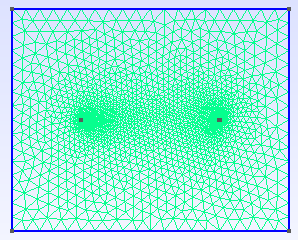
\includegraphics[width=\textwidth]{Image/trous.png}
        \caption{Geometry with wells as circles}
        \label{fig:geo_segments}
    \end{minipage}
    \hfill
    \begin{minipage}[t]{0.48\textwidth}
        \centering
        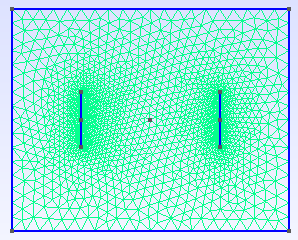
\includegraphics[width=\textwidth]{Image/Line.png}
        \caption{Geometry with wells as segments}
        \label{fig:geo_ronds}
    \end{minipage}
\end{figure}
\subsection{Implementation and Results}
The implementation of this system of equations is done using the finite 
element method (FEM) in Python. You can find the code in the link of the GitHub repository.
\href{https://github.com/chahid-rahouti/Coupled-Thermo-Hydraulic}{https://github.com/chahid-rahouti/Coupled-Thermo-Hydraulic}

\begin{figure}[h!]
    \centering
        \centering
        \includegraphics[width=\textwidth]{Image/solution_couplée.png}
        \caption{Solution of the coupled system of equations for pressure and temperature over time (30 days, 6 mouths, 1 year, 3 years, 10 years)}
        \label{fig:results}
\end{figure}
The results show the evolution of the pressure and temperature in 
the geothermal reservoir over time. The pressure increases in 
the injection well and decreases in the production well, while the temperature 
decreases in the injection well and increases in the production well. 
This behavior is consistent with the expected physics of a geothermal reservoir.(see Figure \ref{fig:results})
I know that the results are not very good, because in the many references i find the distibution
of the pressure and temperature are go to the injection wells to the production wells, but 
in my case the pressure and temperature are not going to the production well. I think there is a problem 
but at this moment I don't know what is the problem. You can see this references (\cite{1}, \cite{2}, \cite{3}, \cite{4}, \cite{5}, \cite{6}).
\section{Conceptual Fault Extension}

\addcontentsline{toc}{chapter}{Bibliography}
\begin{thebibliography}{10}
  \bibitem{1}
  Yuting Luo, Juyan Wei, Meilong Fu, Li Fang, and Xudong L.\\
  \textit{Analysis of Enhanced Geothermal System Reservoir Parameters and Fractures on Heat Recovery Efficiency Based on a Single-Phase Conduction Model.}\\
  Article.

  \bibitem{2}
  Wang Jiwei, Ming Chen, Bo Zhang, et al.\\
  \textit{Numerical Simulation of Hydraulic Fracturing Damage Evolution in Geothermal Reservoirs with Natural Fractures Based on THMD Coupling Model.}\\ 
  Conference Paper, June 2022.\\
  DOI: \href{https://doi.org/10.56952/ARMA-2022-0951}{10.56952/ARMA-2022-0951}.\\
  Available at: \url{https://www.researchgate.net/publication/364247123}
    \bibitem{3}
  Yifan Fan, Shikuan Zhang, Yonghui Huang, Zhonghe Pang, and Hongyan Li.\\
  \textit{Determining the Recoverable Geothermal Resources Using a Numerical Thermo-Hydraulic Coupled Modeling in Geothermal Reservoirs.}\\
  Frontiers in Earth Science, 2022.\\
  Available at: \url{https://www.frontiersin.org/articles/10.3389/feart.2022.XXXXXX}
    \bibitem{4}
  Hua-Peng Chen and Musa D. Aliyu.\\
  \textit{Numerical modelling of coupled thermo-hydraulic problems for long-term geothermal reservoir productivity.}\\
  VII International Conference on Computational Methods for Coupled Problems in Science and Engineering (COUPLED PROBLEMS 2017),\\
  M. Papadrakakis, E. Oñate and B. Schrefler (Eds), 2017.\\
  Department of Engineering Science, University of Greenwich, UK.
    \bibitem{5}
  Musa D. Aliyu and Hua-Peng Chen.\\
  \textit{Numerical modelling of coupled hydro-thermal processes of the Soultz heterogeneous geothermal system.}\\
  ECCOMAS Congress 2016, VII European Congress on Computational Methods in Applied Sciences and Engineering,\\
  M. Papadrakakis, V. Papadopoulos, G. Stefanou, V. Plevris (eds.), Crete Island, Greece, 5–10 June 2016.\\
  Department of Engineering Science, University of Greenwich, UK.
    \bibitem{6}
  S. N. Pandey and Vikram Vishal.\\
  \textit{Sensitivity analysis of coupled processes and parameters on the performance of enhanced geothermal systems.}\\
  Scientific Reports, 7:17057, 2017.\\
  DOI: \href{https://doi.org/10.1038/s41598-017-14273-4}{10.1038/s41598-017-14273-4}.\\
  Available at: \url{https://www.nature.com/articles/s41598-017-14273-4}
\end{thebibliography}

\end{document}
